% The study's challenges
%% The importance of energy and energy storage
En 2019, la consommation mondiale d'énergie finale a doublé par rapport à 1973 et a dépassé la barre des \qty{400}{\exa \joule}, dont \qty{19.7}{\percent} d'électricité \cite{birol_key_nodate}.\\
Il est donc nécessaire de pouvoir stocker efficacement l'énergie produite, c'est-à-dire avec un minimum de pertes, une grande capacité de stockage, et des temps de charge et de décharge courts.

%% The interest, usages and challenges of SCs
Les supercondensateurs sont des systèmes de stockage d'énergie caractérisé par une haute densité de puissance. À l'inverse des condensateurs habituels, ils sont capables de stocker de plus grandes quantités d'énergie.
Bien que leurs réserves soient bien loin des batteries, ils ont l'avantage de pouvoir se charger ou se décharger bien plus rapidement.\\
Ceci explique donc leur utilisation répandue pour les véhicules électriques, systèmes d'alimentation sans fil ou encore appareils portables.\\
Enfin, malgré le nombre d'études ayant déjà été menées, le fonctionnement de ces appareils reste encore peu compris. Ainsi, nous suivons une piste sérieuse\cite{bo_design_2018} pour approfondir notre compréhension avec les simulations de Dynamique Moléculaire d'électrodes capacitives.

%% Describing the SCs
Les supercondensateurs sont composés d'électrodes poreuses séparées par une membrane perméable et plongées dans un électrolyte. Ceci permet le déplacement des charges d'une électrode à l'autre lorsque l'appareil est en charge ou en décharge (\autoref{fig:schema_supercondensateur}).

\begin{figure}[hb]
    \centering
    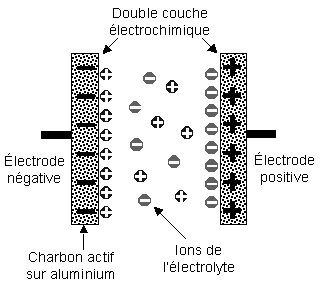
\includegraphics[height=5cm]{supercondensateur.png}
    \caption{Schéma d'un supercondensateur}
    \label{fig:schema_supercondensateur}
\end{figure}

Les électrodes capacitives sont généralement constituées de charbon actif : la porosité de telles électrodes permet d'augmenter la surface de contact avec l'électrolyte pour atteindre des capacitance spécifique de \qtyrange[range-units = single]{100}{300}{\farad \per \gram}.\\
Quant aux électrolytes, ils peuvent être groupés en fonction de leur nature : aqueux, organiques et ioniques. Parmi les électrolytes aqueux se démarquent\cite{zhong_review_2015} les électrolytes acides (\ce{H2SO4}), alkalins (\ce{KOH}), et neutres (\ce{Na2SO4}).

% Presenting the methods and tools
%% Molecular Dynamics and LAMMPS
Lors de cette étude, nous utilisons \emph{Large Atomic/Molecular Massively Parallel Simulator} (LAMMPS) pour effectuer des simulations de Dynamique Moléculaire. En effet, cet outil permet de mettre en place des simulations et d'en contrôler les conditions relativement facilement (contrôle du/des potentiel/s, de l'ensemble thermodynamique, thermostat, barostat, etc.).
%% The data extracting and processing task
Aussi, l'extraction et le traitement des données de simulations ont été une tâche non-négligeable. Pour cela, nous avons utilisé majoritairement des programmes écrits en C dont la conception et réalisation sont détaillées en annexes.\\
%% The additionnal tools
Enfin, pour des outils supplémentaires ont été utilisés pour les tâches restantes comme la visualisation des trajectoires\cite{ovito} ou encore la réalisation de configurations initiales\cite{martinez_packmol_2009}.

% Presenting the plan
La structure des électrodes capacitives étant très complexe du fait du grand nombre de pores et de leur diversité, nous avons préféré adopter un système modèle, que nous présentons en première section.\\
Puis, nous présenterons les outils que nous utilisons pour simuler un supercondensateur en charge, à savoir le potentiel réactif \emph{ReaxFF}\cite{van_duin_reaxff_2001}\cite{russo_atomistic-scale_2011}\cite{senftle_reaxff_2016} et \emph{EChemDID}\cite{onofrio_voltage_2015}.\\
Enfin, nous présentons les résultats obtenus et observations faites lors de cette étude, notamment par rapport à l'adsorption des ions à la surface des électrodes et la répartition des charges en leur sein.
